
\documentclass[12pt,letterpaper]{article}


\usepackage[top=1in, 
		    bottom=1in,
		    left=1in,
		    right=1in]{geometry}
\usepackage{setspace}	% makes the \singlespacing, \onehalfspacing, and \doublespacing commands available
% \usepackage[en-US]{datetime2}
% \DTMlangsetup{showdayofmonth=false}
% \usepackage{titlesec}
\usepackage{listings}	% allows for placing programming code to be displayed correctly
\usepackage{siunitx}	% units
\usepackage{amsmath}
\usepackage{amsfonts}
\usepackage{amssymb}
\usepackage{graphicx}
\usepackage{booktabs}
\usepackage{multirow}
\usepackage{pgfplots}
\pgfplotsset{compat=newest}
\usepackage{tikz}
%\usetikzlibrary{shapes.geometric}
% \usepgfplotslibrary{external} 
% \tikzexternalize[prefix=pdfimages/,
% 		        mode=list and make]
\usepackage{caption}
\usepackage[list=true,
		     listformat=simple]{subcaption}
%\usepackage{cleveref}	% this should really go last
% \usepackage[colorlinks,
% 		     linkcolor=black,
% 		     citecolor=black,
% 		     plainpages=false,
% 		     pdfpagelabels]{hyperref}
% \usepackage[all]{hypcap}
\usepackage{cleveref}
% \doublespacing

\pagenumbering{gobble}
\newcommand{\mymder}[2]{\ensuremath{\frac{\mathrm{D}#1}{\mathrm{D}#2}}}
\newcommand{\mypder}[2]{\ensuremath{\frac{\partial #1}{\partial #2}}}
\newcommand{\mypdertwo}[2]{\ensuremath{\frac{\partial^2 #1}{\partial #2^2}}}
\newcommand{\mymdervec}[1]{\ensuremath{mypder{#1}{t} + }}
\newcommand{\myder}[2]{\ensuremath{\frac{d#1}{d#2}}}
\newcommand{\mydiv}[1]{\ensuremath{\nabla \cdot {#1}}}
\newcommand{\myfrac}[2]{\ensuremath{^{#1}\!/_{#2}}}
\newcommand{\myfunc}[2]{\ensuremath{#1 \left( #2 \right)}}
\newcommand{\myparen}[1]{\ensuremath{\left( #1 \right)}}
\newcommand{\mybrack}[1]{\ensuremath{\left[ #1 \right]}}
\newcommand{\mybrace}[1]{\ensuremath{\left\{ #1 \right\}}}
\newcommand{\mysin}[1]{\ensuremath{\myfunc{\mathrm{sin}}{#1}}}
\newcommand{\mycos}[1]{\ensuremath{\myfunc{\mathrm{cos}}{#1}}}
\newcommand{\myexp}[1]{\ensuremath{\myfunc{\mathrm{exp}}{#1}}}
\newcommand{\myint}[4]{\ensuremath{\int_{#1}^{#2} {#3} d {#4}}}


\newcommand{\Rld}{\ensuremath{\mathit{Re}}}
\newcommand{\St}{\ensuremath{\mathit{St}}}
\newcommand{\Prn}{\ensuremath{\mathit{Pr}}}
\newcommand{\Sc}{\ensuremath{\mathit{Sc}}}
\newcommand{\Sh}{\ensuremath{\mathit{Sh}}}
\newcommand{\Nu}{\ensuremath{\mathit{Nu}}}
\newcommand{\Bi}{\ensuremath{\mathit{Bi}}}


\let\textacute\'
\let\textgrave\`


\newcommand{\includetikz}[2]{%
    \tikzsetnextfilename{#2}%
    \input{#1#2.tex}%
}

\begin{document}

\noindent
NAME:

\noindent
MECH 131A Midterm

\noindent
Date: October $31^{\mathrm{st}}$, 2024

\subsection*{Midterm Questions}

\begin{enumerate}

    %% Non-dimensional numbers
    \item Give a brief description of the following non-dimensional numbers.
        Describe what they mean and what they indicate for a physical situation.

    \begin{enumerate}
        \item $\Bi = \frac{h L}{k}$ \\ \\ \\ \\ \\ \\ \\ \\
        \item $\Rld = \frac{u L}{\nu}$ \\ \\ \\ \\ \\ \\ \\ \\
        % \item $\Prn = \frac{\nu}{\alpha}$ \\ \\ \\ \\ \\ \\ \\ \\
        \item $\St = \frac{h}{\rho c_p u}$ \\ \\ \\ \\ \\ \\ \\
    \end{enumerate}
    \newpage

    %% Lumped Capacitance
    \item Hot small steel balls are quenched in an cool oil bath with a small $\Bi$.
    \begin{enumerate}
        \item Sketch how the dimensionless temperature changes with dimensionless time. \\ \\ \\ \\ \\ \\ \\ \\ \\ \\ \\ \\ \\ \\ \\ \\ \\ \\ \\ \\
        \item If a pump is suddenly turned on two time constants into the quenching process, suddenly doubling the heat transfer coefficient, graph the new dimensionless temperature profile.
    \end{enumerate}
    \newpage

    %% Semi-infinite conduction
    \item A rocket is sitting on the pad ready to launch.
        Before launch, the propellants are saturated at atmospheric pressure, but close to launch the tanks are suddenly pressurized. % so the pump at the bottom of the tank has the correct inlet pressure.
        The pressure remains elevated until the end of the mission.
        
    \begin{enumerate}
        \item In terms of a pressure increase, $\Delta P$, describe the temperature profile after launch.
            The Clausius-Clapeyron equation describes how the sudden temperature change \textit{at the surface} is related to the sudden pressure increase:
            
            \begin{equation*}
                \frac{d P}{d T} = \frac{h_{fg} P}{T R^2} \to \mathrm{ln} \left( \frac{P_1 + \Delta P}{P_1} \right) = \frac{h_{fg}}{R^2} \left( \frac{1}{T_1} - \frac{1}{T_1 + \Delta T} \right)
            \end{equation*}

            Sketch several temperature curves as a function of distance from the liquid surface towards the bottom of the tank at various times \textit{if there is no circulation of the liquid within the tank}.
            You can assume the liquid height is very long compared to the region affected by the sudden temperature increase at the liquid surface.
        \newpage
        \item Approximately how far will the step change in surface temperature penetrate into the liquid 4 minutes into flight?
    \end{enumerate}
    \newpage

    %% Forced convection
    \item Fluid velocities can be measured with a constant temperature hot-wire anemometer.
        A long ($\sim \SI{1.25}{\milli\meter}$), fine wire ($\sim \SI{4}{\micro\meter}$ diameter), supported between two much larger needles, is connected to an electronic circuit that maintains a constant resistance, $R_w$, by adjusting the voltage, $V_w$.
        The electrical power dissipated in the wire, $V_w^2 / R_w$, is convected away by the surface of the wire.
        Show that
        \begin{equation*}
            V_w^2 = \left( T_w - T_\infty \right) \left( A + B u^{1/2} \right)
        \end{equation*}
        and provide estimates of $A$ and $B$.
        Note that the kinematic viscosity of air, $\nu$, is approximately \SI{15e-6}{\square\meter\per\second}.
        Start by estimating the approximate size of $\Rld_D$.
    \newpage
    
    \item Two thin planes, with width and depth of $W$ and $L$, of dissimilar materials are glued together horizontally along their thin faces, of thickness $t$, with a heating element in between them that generates $q'' $ (\si{\watt\per\square\meter}).
    	This results in a single thin plate of dimensions $2 W$ by $L$ with a heating element running through the middle, scrunched between the two faces of $t$ thickness.
    	You can assume the heater is very thin and has no contact resistance with the two thin planes.
    
    \begin{enumerate}
        \item Give the solution for the temperature profiles if both materials are exposed to the same heat transfer coefficient.
        \newpage
        \item Describe how the temperature profiles change if instead of the heat transfer coefficient being constant for all surfaces, a fluid flows normal to the joining line.
%        \item Describe how the temperature profiles change if if instead of the heat transfer coefficient being constant for all surfaces, a fluid flows parallel to the joining line. 
    \end{enumerate}
    \newpage

%    \item An array of parallel rectangular fins are used to increase heat transfer from a heated surface to the ambient air flow with separation between the fins of $w$.
%        About how long should the fins be in the direction of the flow before the fin performance starts degrading?
%        Note, the air is moving parallel with the base of the fins, not towards the base of the fins.
%        You can assume the effective free stream velocity of the flow does not change in the streamwise direction for this problem.
%        Give your answer for both fully laminar flow and flow that is tripped into turbulence at the leading edge so it is turbulent for the whole flow length.
%    \newpage
\end{enumerate}

~
\newpage
~
\newpage
~
\newpage
~
\newpage
~
\newpage
~
\newpage

\subsection*{Useful Equations}

\subsubsection*{Basic Transport Equations}

\begin{figure}[!htpb]
    \centering
    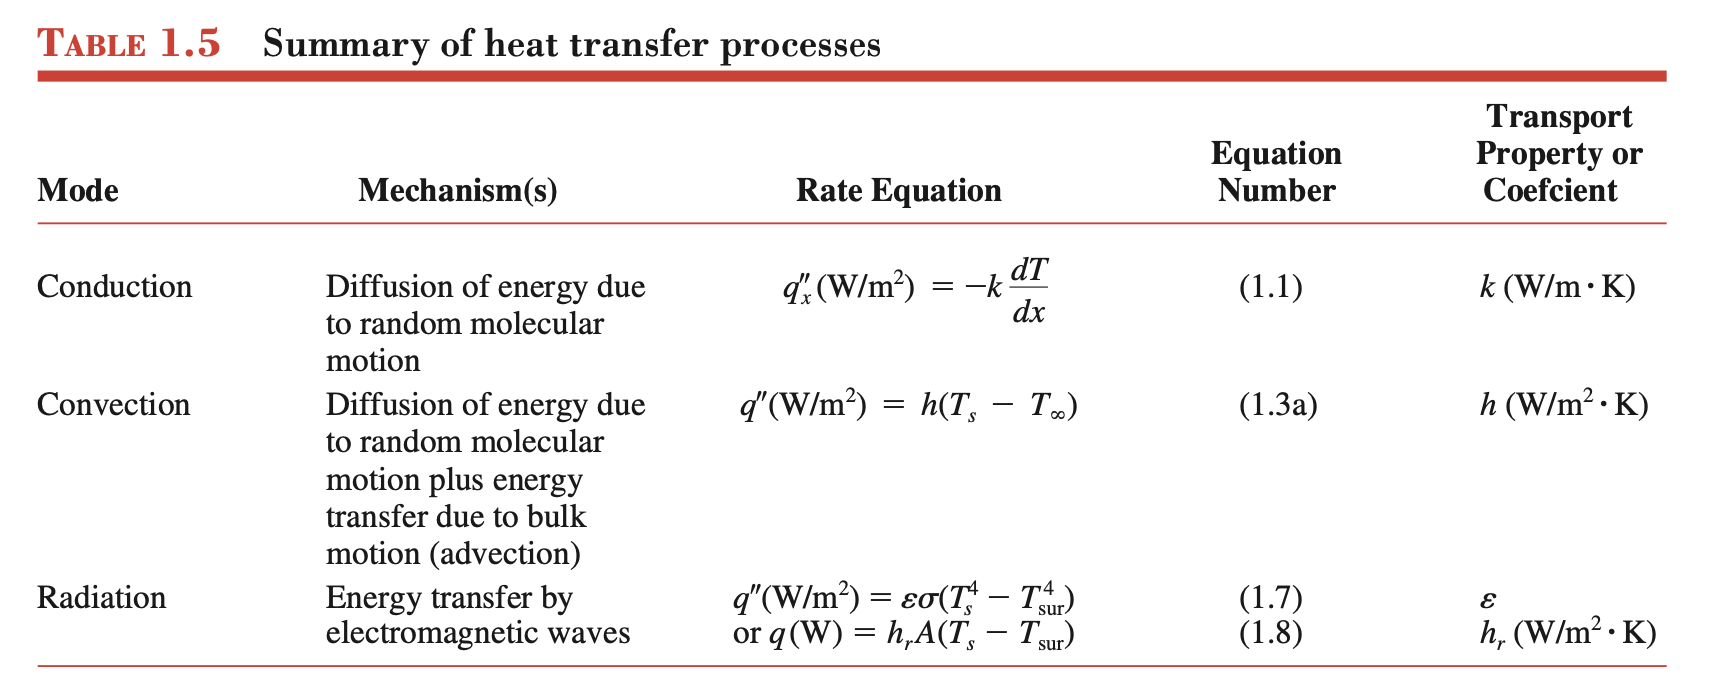
\includegraphics[width=0.95\linewidth]{./image10.png}
\end{figure}


\clearpage
\subsubsection*{Conduction Equation}

\begin{figure}[!htpb]
    \centering
    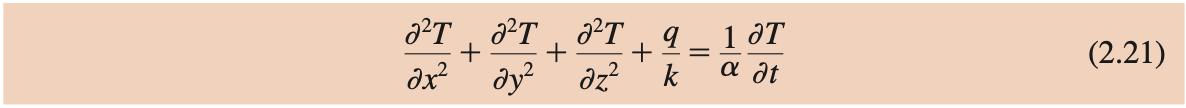
\includegraphics[width=0.95\linewidth]{./image20.png}
\end{figure}

\begin{figure}[!htpb]
    \centering
    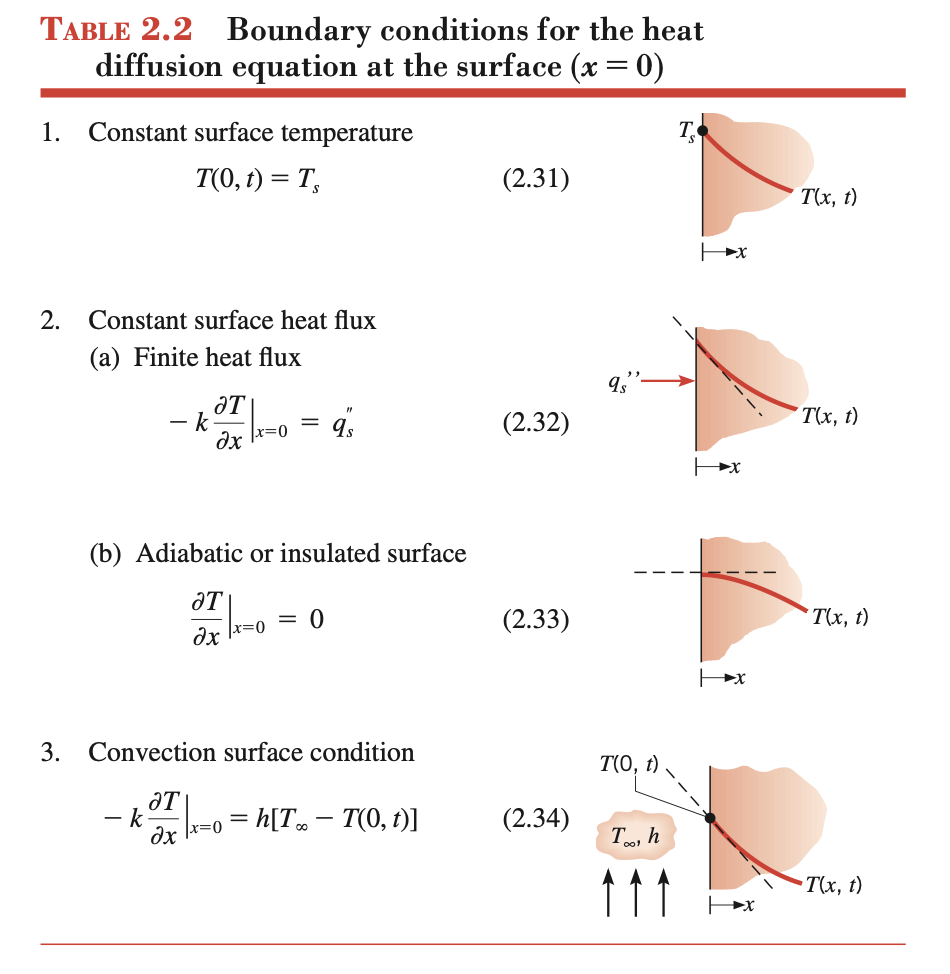
\includegraphics[width=0.95\linewidth]{./image21.png}
\end{figure}



\clearpage
\subsubsection*{Steady State Solutions}

\begin{figure}[!htpb]
    \centering
    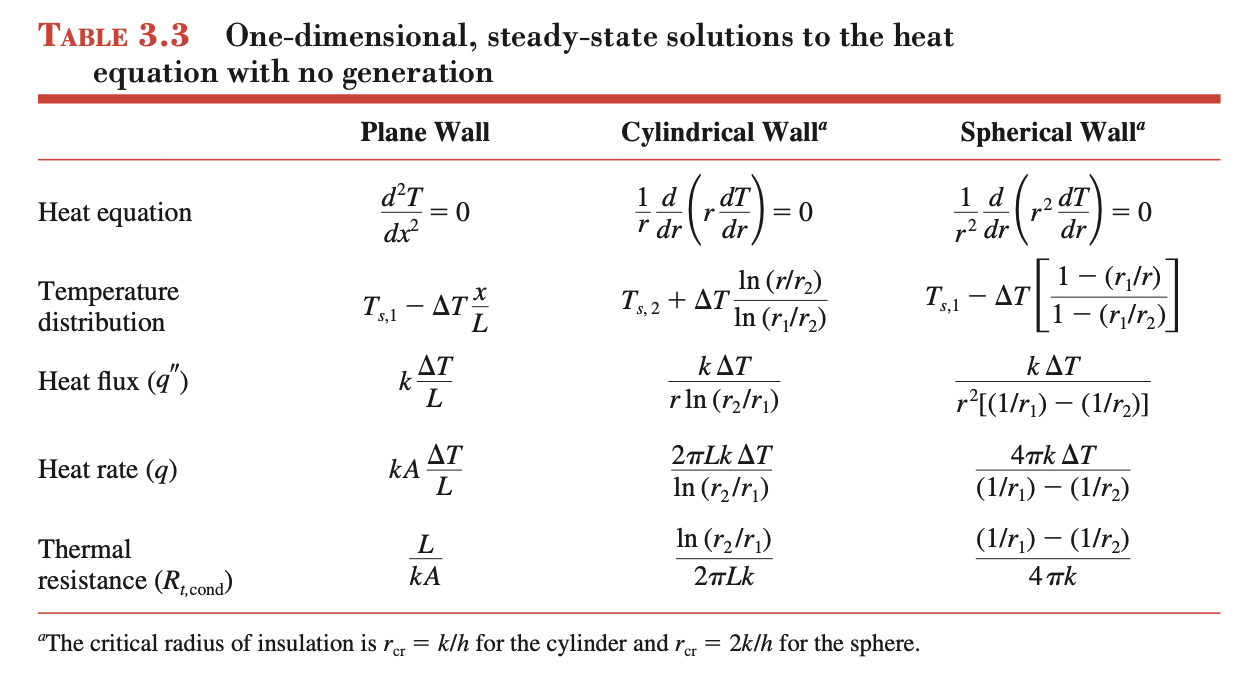
\includegraphics[width=0.95\linewidth]{./image30.png}
\end{figure}


\clearpage
\subsubsection*{Fin Equations}

\begin{figure}[!htpb]
    \centering
    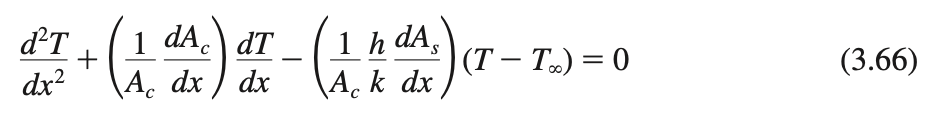
\includegraphics[width=0.95\linewidth]{./image31a.png}
\end{figure}

\begin{figure}[!htpb]
    \centering
    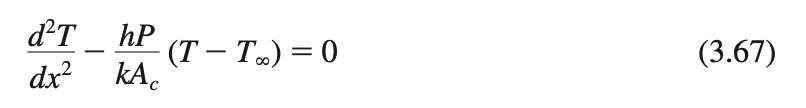
\includegraphics[width=0.95\linewidth]{./image31b.png}
\end{figure}

\begin{figure}[!htpb]
    \centering
    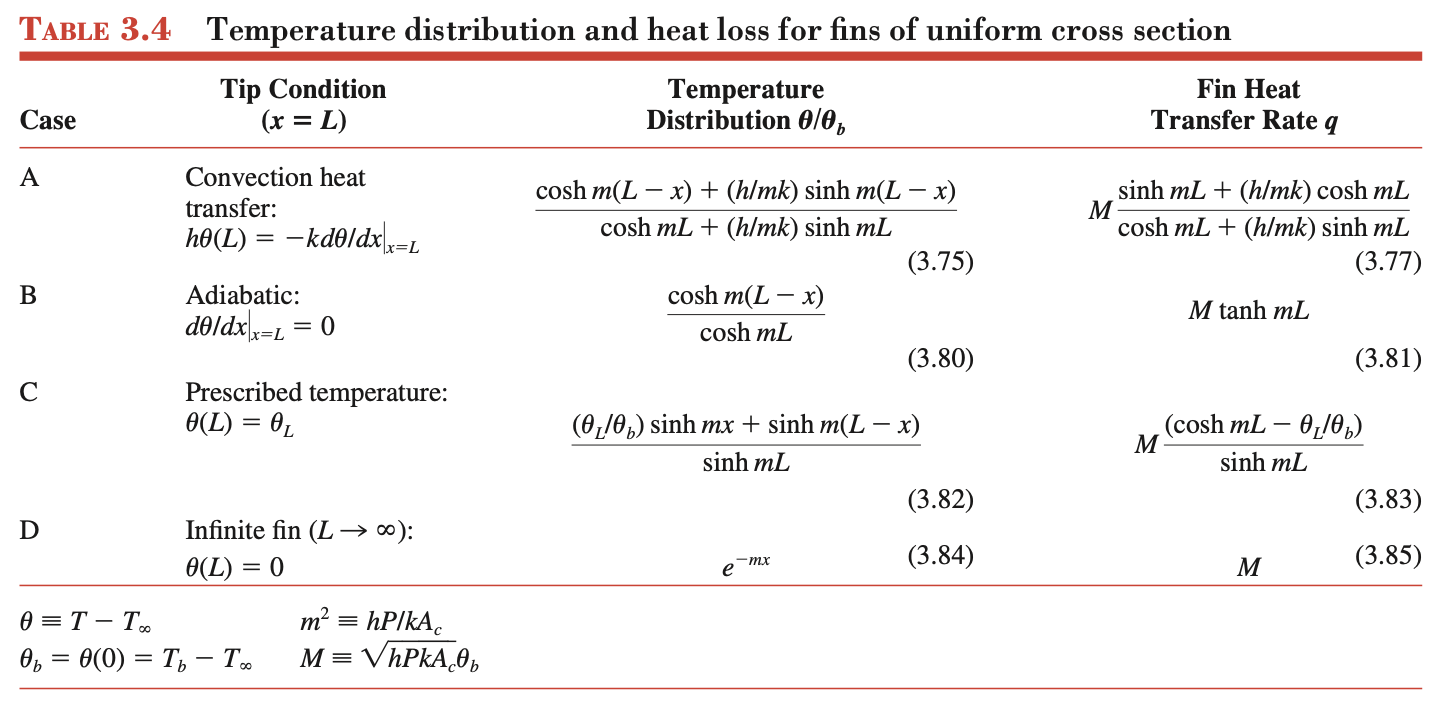
\includegraphics[width=0.95\linewidth]{./image32.png}
\end{figure}

\begin{equation*}
	y'' + m^2 y = 0 \to y = c_1 \mysin{m x} + c_2 \mycos{m x}
\end{equation*}

\begin{equation*}
	y'' - m^2 y = 0 \to y = c_1 \myexp{m x} + c_2 \myexp{ - m x}
\end{equation*}


\clearpage
\subsubsection*{Transient Conduction}

\begin{figure}[!htpb]
    \centering
    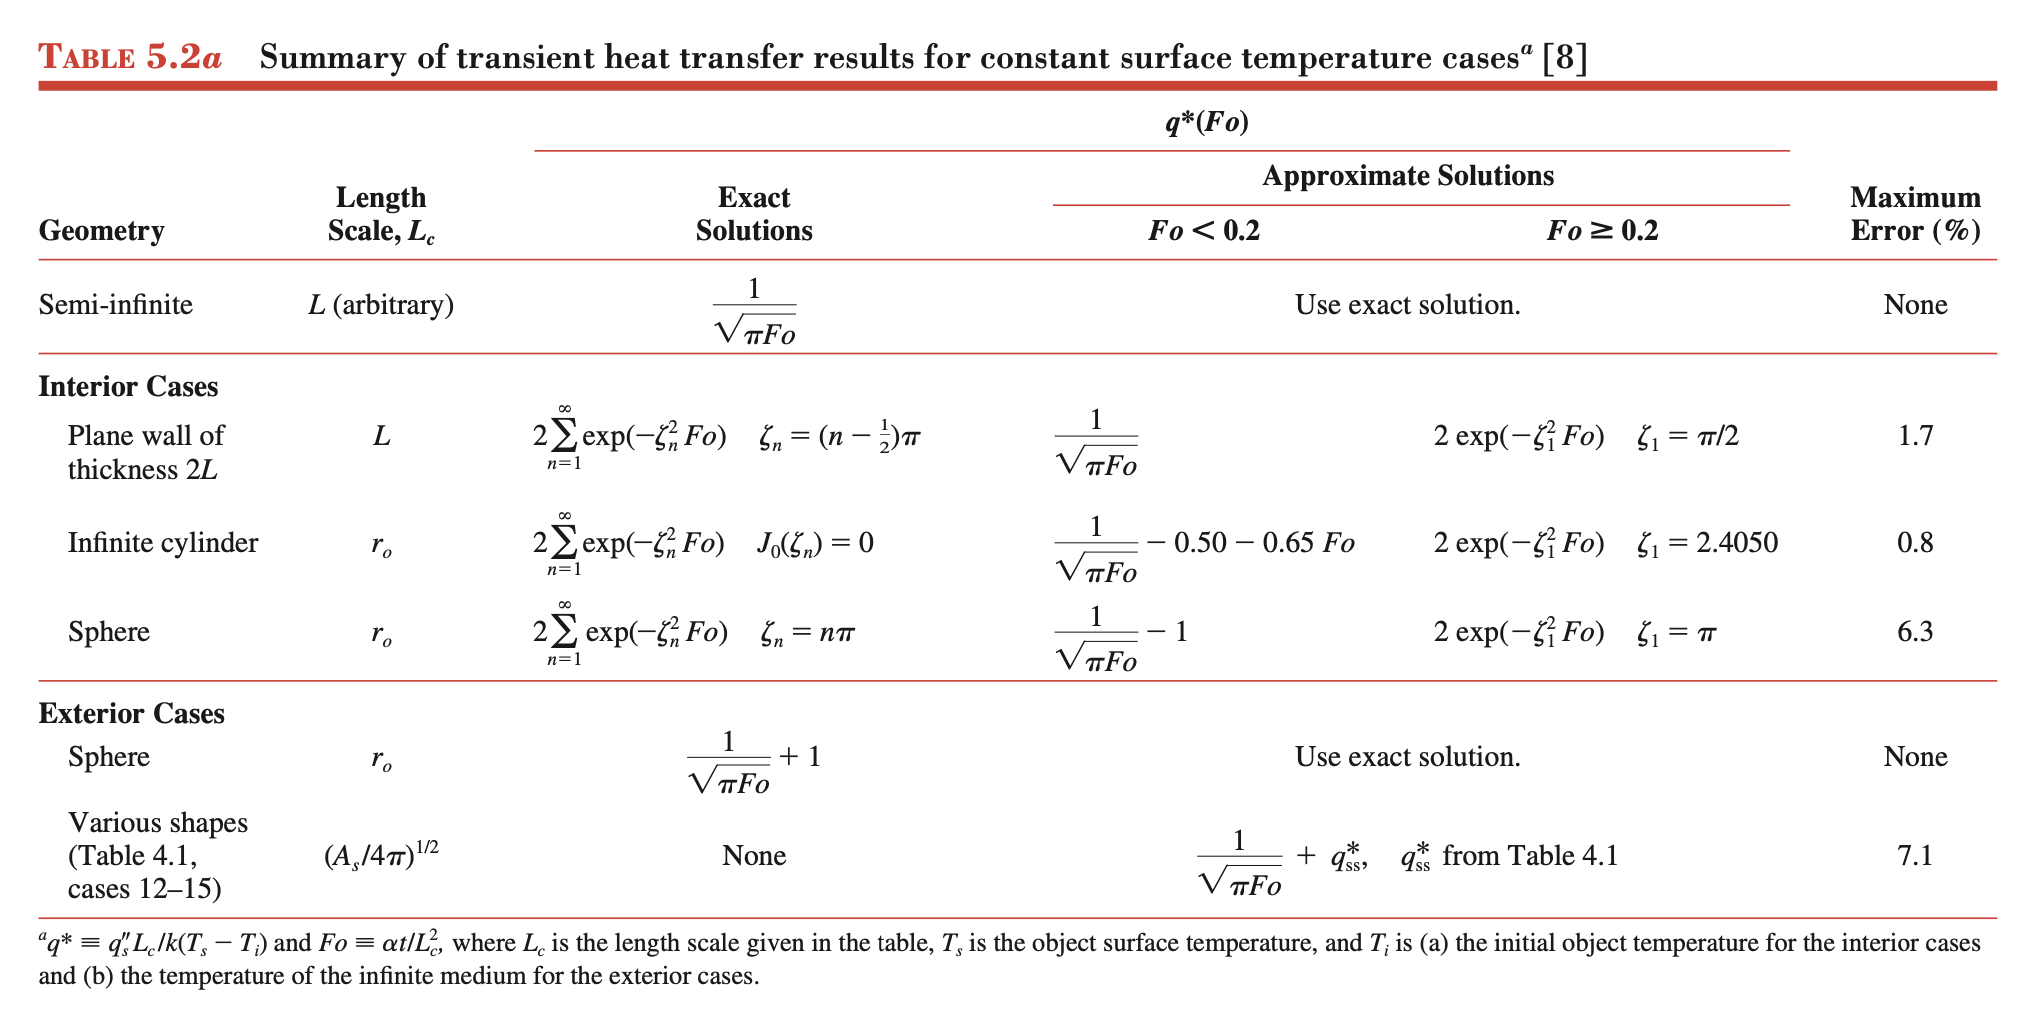
\includegraphics[width=0.95\linewidth]{./image50.png}
\end{figure}

\begin{figure}[!htpb]
    \centering
    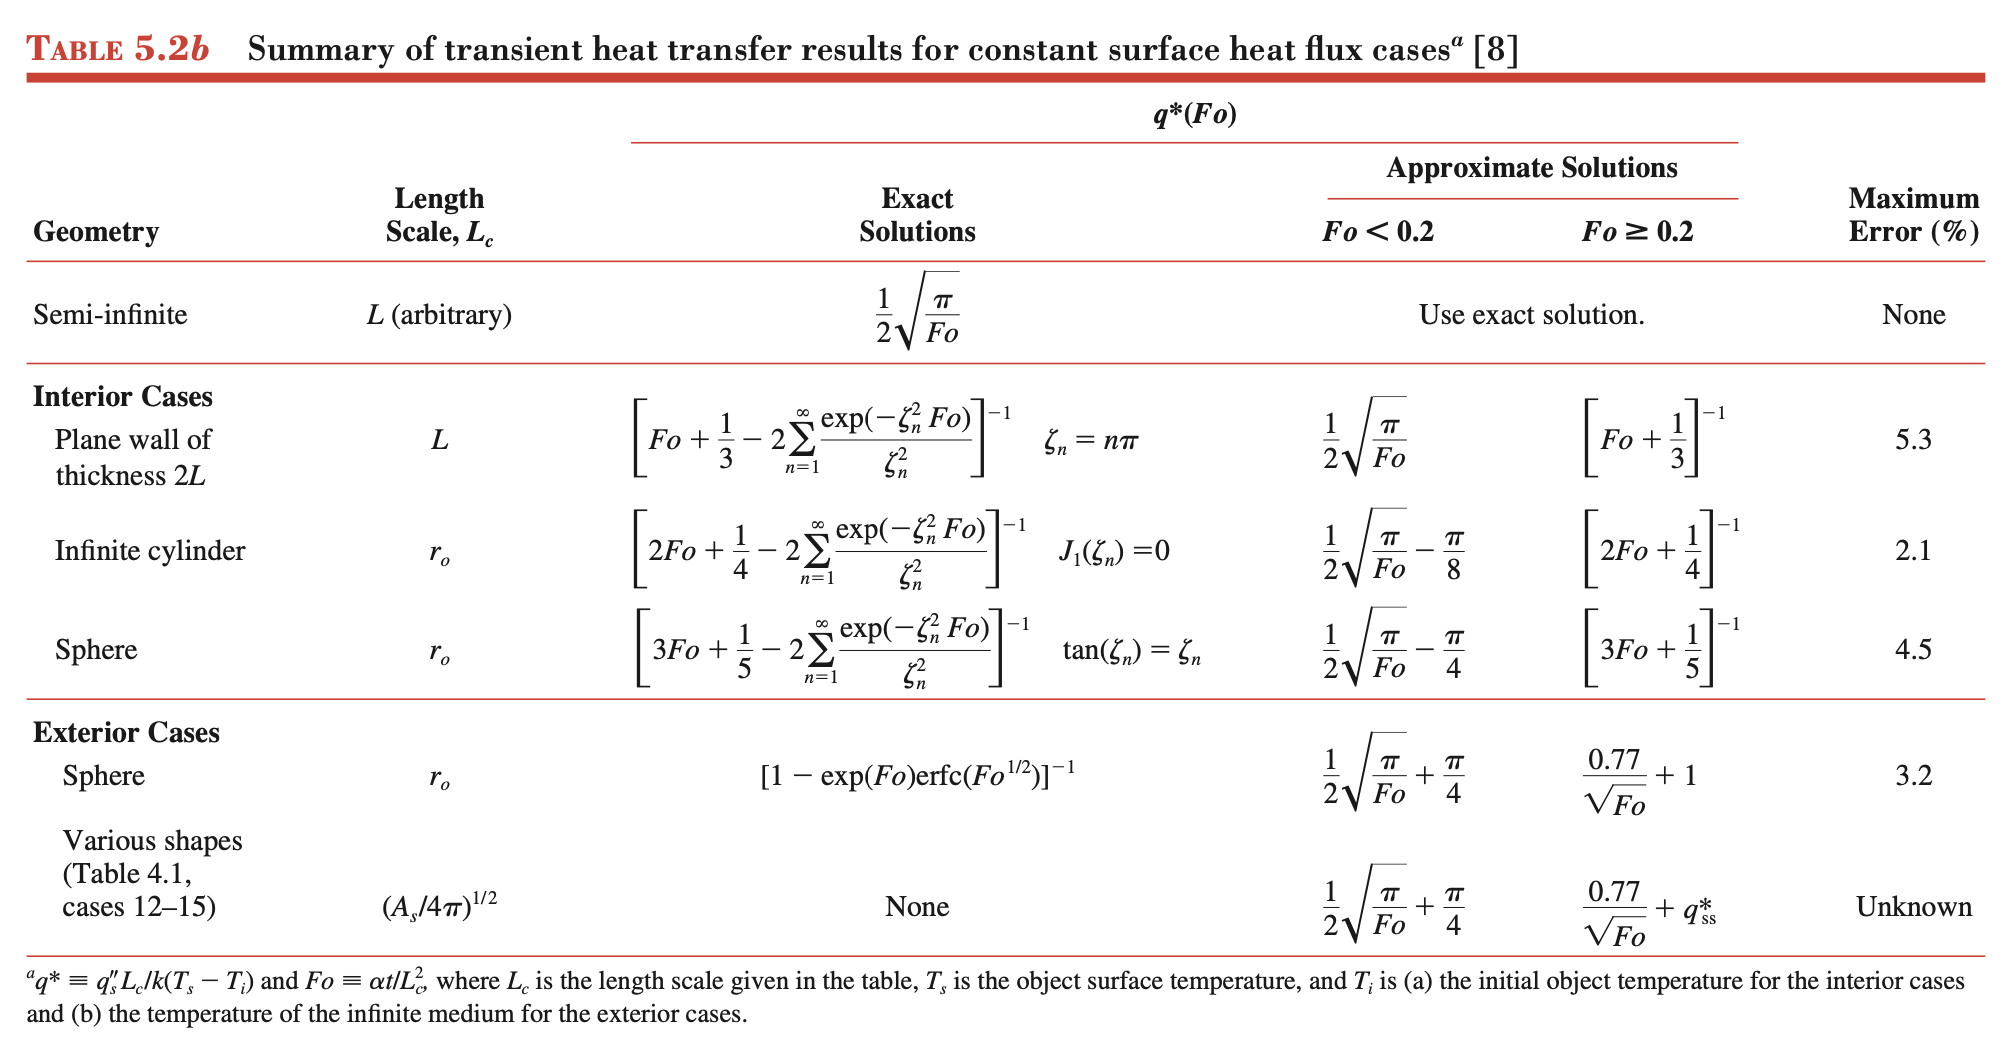
\includegraphics[width=0.95\linewidth]{./image51.png}
\end{figure}

% \begin{figure}[!htpb]
%     \centering
%     \includegraphics[width=0.95\linewidth]{./image52.png}
% \end{figure}

\begin{figure}[!htpb]
    \centering
    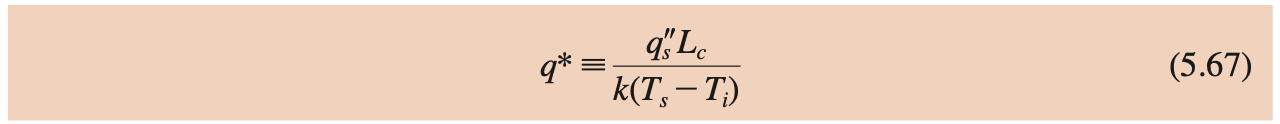
\includegraphics[width=0.95\linewidth]{./image53.png}
\end{figure}


\clearpage
\subsubsection*{Transient Semi-Infinite Solutions}

\begin{figure}[!htpb]
    \centering
    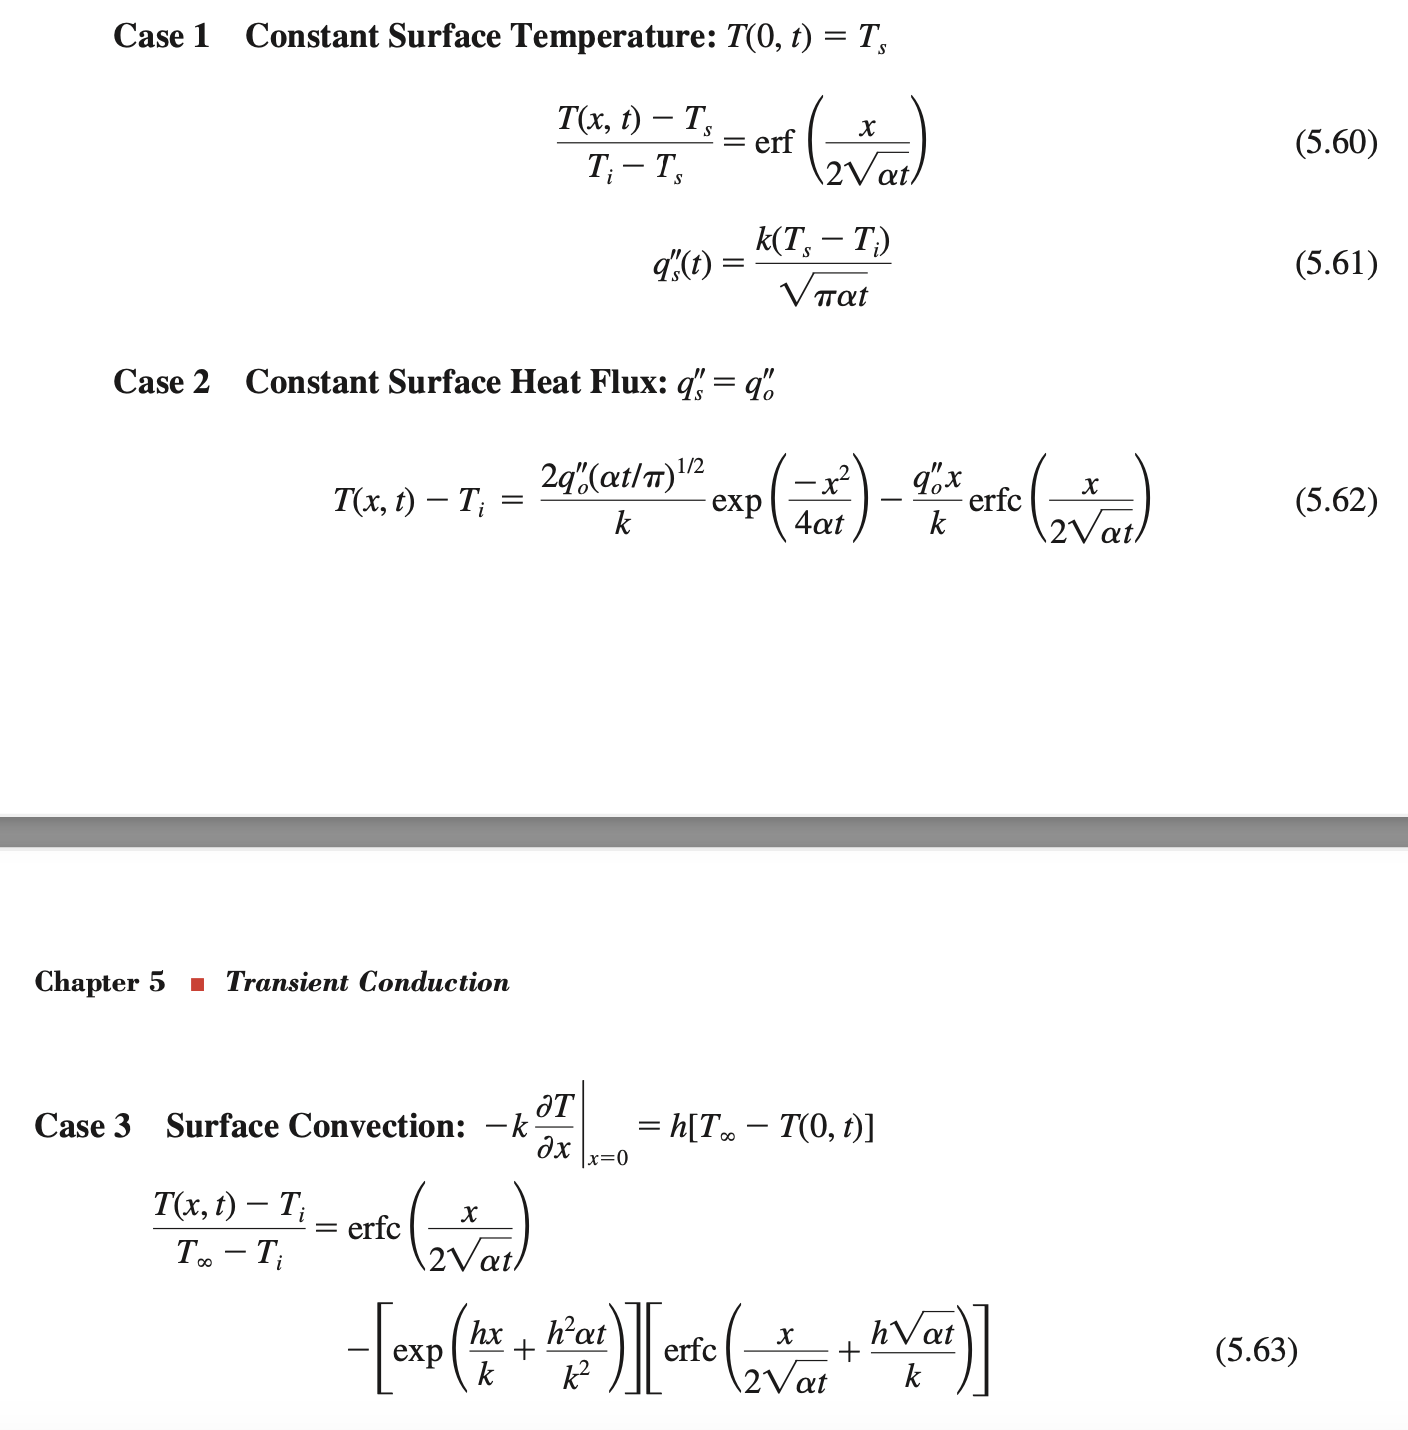
\includegraphics[width=0.95\linewidth]{./image54.png}
\end{figure}


\clearpage
\subsubsection*{Convection Correlations}

\begin{figure}[!htpb]
    \centering
    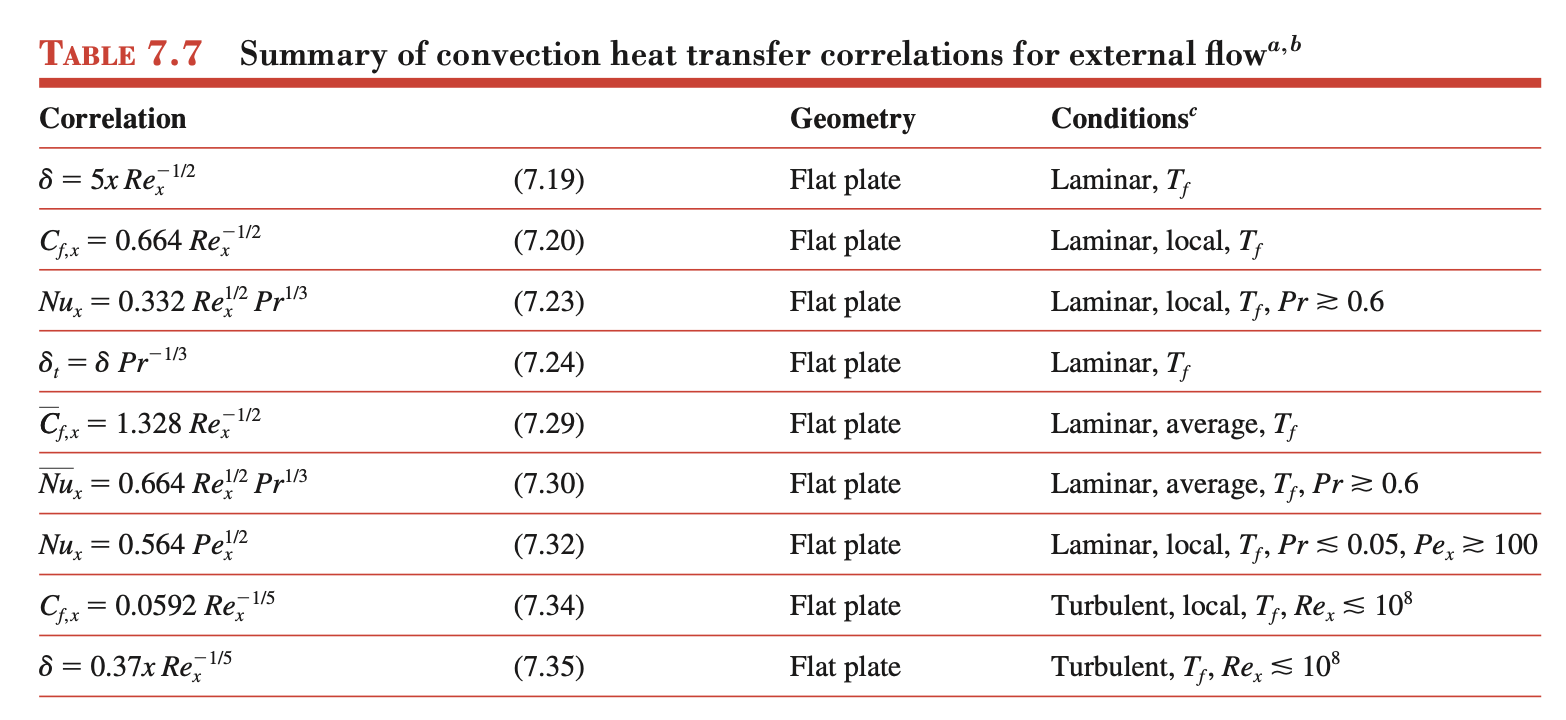
\includegraphics[width=0.95\linewidth]{./image70.png}
\end{figure}

\begin{figure}[!htpb]
    \centering
    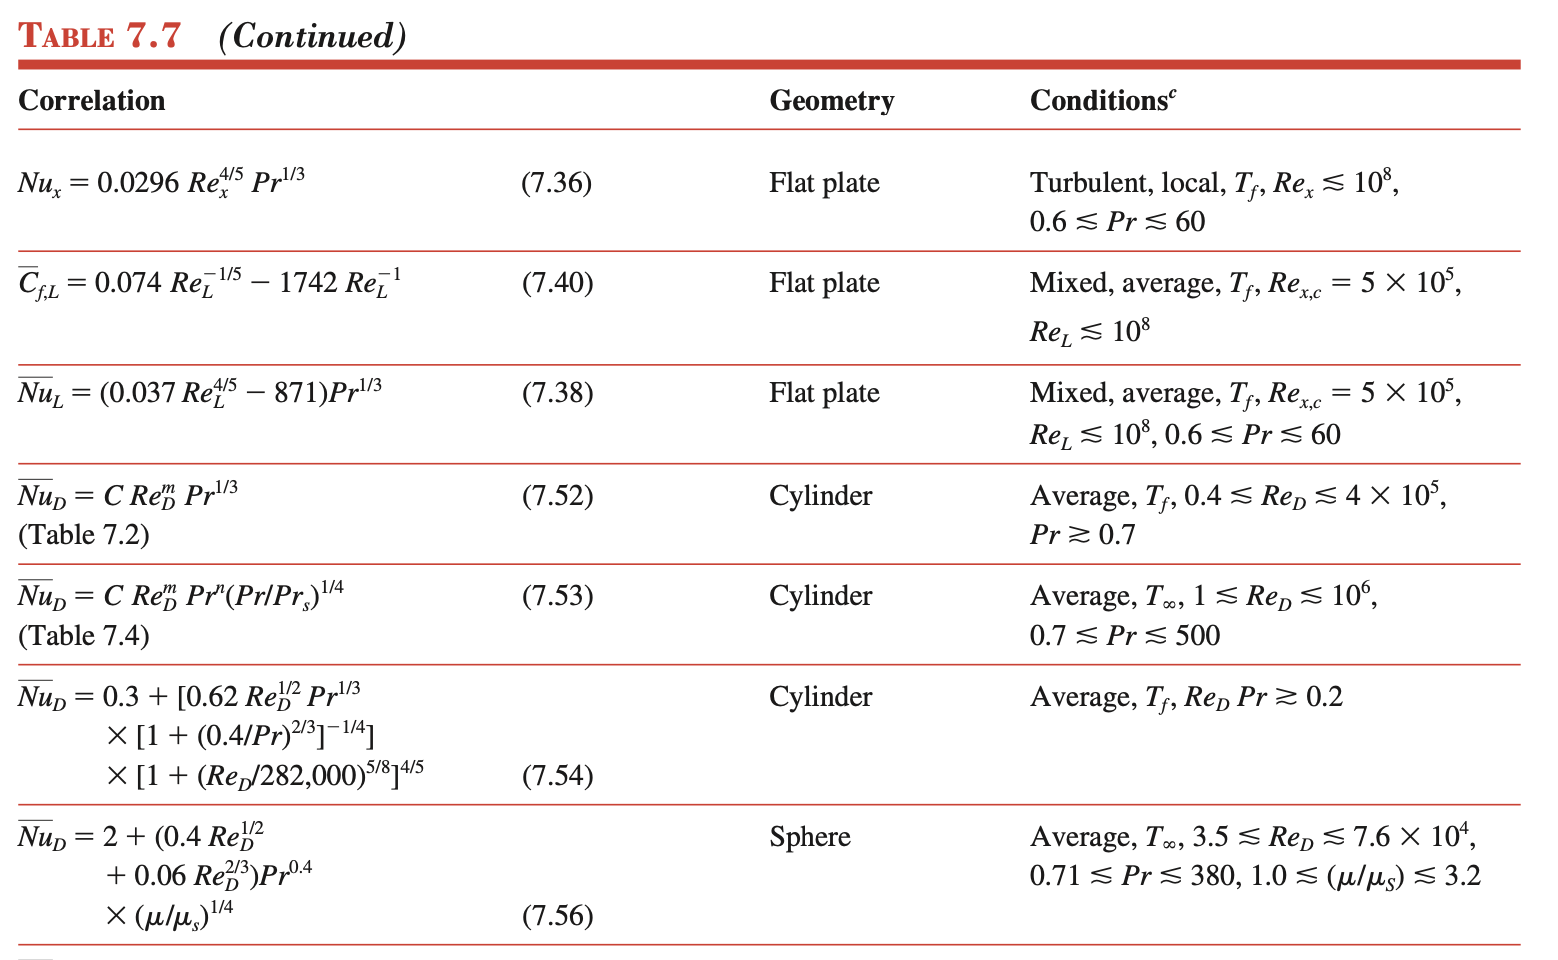
\includegraphics[width=0.95\linewidth]{./image71.png}
\end{figure}

\end{document}
